\subsection{Pengujian Pengiriman Citra Kamera pada Robot di Simulasi}
\label{subsec:citrasimulasi}

\begin{figure}[ht]
  \centering
  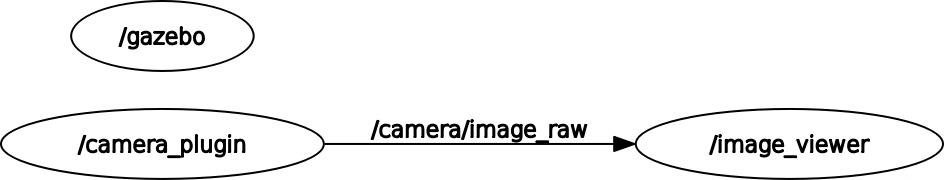
\includegraphics[width=0.8\textwidth,keepaspectratio]{gambar/rosgraph-camera-plugin.png}
  \caption{Relasi antar-\emph{node} dari pengujian pengiriman citra kamera di simulasi.}
  \label{fig:rosgraphcameraplugin}
\end{figure}

Pengujian pengiriman citra kamera pada robot di simulasi dilakukan dengan cara menjalankan lingkungan \emph{indoor} pada simulator gazebo,
  menjalankan \emph{image viewer node} untuk melihat hasil pengiriman gambar,
  serta menjalankan \emph{command-line} \lstinline{$ ros2 topic delay} dan \lstinline{$ ros2 topic hz} untuk mengukur \emph{delay} serta frekuensi dari data yang dikirim.
Seperti yang terlihat pada gambar \ref{fig:rosgraphcameraplugin},
  \emph{node} \lstinline{/camera_plugin} akan mengirimkan \emph{topic} \lstinline{/camera/image_raw} yang berisi citra kamera,
  setelah itu \emph{node} \lstinline{/image_viewer} akan menerima citra tersebut dan menampilkannya dalam bentuk GUI.

Pengujian ini dilakukan dengan berbagai macam konfigurasi resolusi citra yang dikirim.
Hasil pengujian ini bisa dilihat pada tabel \ref{tb:pengirimancitrasimulasi}.
Pada tabel tersebut \emph{width} dan \emph{height} merupakan resolusi citra yang dikirimkan,
  \emph{size} merupakan hasil perkalian resolusi dengan jumlah \emph{channel} (dalam hal ini 4 untuk citra RGBA),
  \emph{delay} merupakan selang waktu yang dibutuhkan sebelum citra sampai ke penerima,
  dan \emph{rate} merupakan frekuensi pengiriman citra.

\begin{longtable}{|c|c|c|c|c|c|}
  \caption{Hasil \emph{delay} dan frekuensi dari pengiriman citra kamera pada robot di simulasi.}
  \label{tb:pengirimancitrasimulasi}
  \\ \hline \rowcolor[HTML]{E0E0E0}
  \multicolumn{3}{|c|}{Resolution} &
  \multicolumn{1}{|c|}{Delay} &
  \multicolumn{2}{|c|}{Rate}
  \\ \hline \rowcolor[HTML]{E0E0E0}
  Width & Height & Size (KB) & ms & hz & percent
  \csvreader[head to column names]{data/pengiriman_citra_simulasi.csv}{}{
    \\ \hline
    \width & \height & \size & \delay & \rate & \ratepercent
  }
  \\ \hline
\end{longtable}


Seperti yang dapat dilihat pada gambar \ref{fig:grafikpengirimancitrasimulasi},
  dari data yang dihasilkan oleh pengujian ini dapat diketahui bahwa semakin besar ukuran data yang dikirimkan,
  maka \emph{delay} akan cenderung naik dan frekuensi akan cenderung turun.
Pada pengujian ini, dapat diketahui agar \emph{delay} dan frekuensi yang dihasilkan stabil,
  data yang dikirimkan hendaknya ada di bawah 1000 KB (dalam hal ini adalah citra dengan resolusi 640x480),
  karena pada titik itu frekuensi yang dikirimkan tidak jauh berbeda dari frekuensi citra yang ditangkap oleh kamera yang ada di simulasi, yakni 30 FPS.


\begin{figure}[ht]
  \centering
  \begin{tikzpicture}
    \begin{axis}[
        height=0.38\textwidth,
        width=0.9\textwidth,
        ylabel=Delay (ms),
        ymajorgrids,
        ymin=0,
        ymax=125,
      ]
      \addplot table[x=size,y=delay,col sep=comma]{data/pengiriman_citra_simulasi.csv};
    \end{axis}
  \end{tikzpicture}
  \begin{tikzpicture}
    \begin{axis}[
        height=0.38\textwidth,
        width=0.9\textwidth,
        xlabel=Data Size (KB),
        ylabel=Rate (hz),
        ymajorgrids,
        ymin=0,
        ymax=40,
      ]
      \addplot table[x=size,y=rate,col sep=comma]{data/pengiriman_citra_simulasi.csv};
    \end{axis}
  \end{tikzpicture}
  \caption{Grafik \emph{delay} dan frekuensi dari pengiriman citra pada robot di simulasi.}
  \label{fig:grafikpengirimancitrasimulasi}
\end{figure}

